% ArtiOODBench --- NeurIPS Datasets and Benchmarks Track submission.
%
% Build note: this file expects the official NeurIPS 2024 style file
% `neurips_2024.sty` to be present in the same directory (download from
% https://neurips.cc/). The line below loads it. If the style file is not
% available, comment out the \usepackage{neurips_2024} line and uncomment the
% \documentclass{article} fallback block immediately under it to compile a
% plain-article preview.
%
% All numerical values are verifier-confirmed against the held-out protocol
% (see project 02_ACCEPTANCE.md v6 and 05_DRAFT_core.md). No number is invented.

\documentclass{article}

% --- NeurIPS 2024 D&B style (preferred) -------------------------------------
\usepackage[final]{neurips_2024}     % requires neurips_2024.sty in this folder
% --- Fallback (uncomment the three lines below and comment the line above if
%     neurips_2024.sty is unavailable). The NeurIPS style loads natbib itself;
%     the fallback must load it explicitly so that \citep resolves. -----------
% \usepackage[margin=1in]{geometry}
% \usepackage{parskip}
% \usepackage[numbers]{natbib}

\usepackage[utf8]{inputenc}
\usepackage[T1]{fontenc}
\usepackage{hyperref}
\usepackage{url}
\usepackage{booktabs}
\usepackage{amsmath}
\usepackage{amssymb}
\usepackage{graphicx}
\usepackage{xcolor}

\title{ArtiOODBench: Auditing What Out-of-Distribution Detectors Actually
Measure on Cross-Institution Medical-Imaging Benchmarks}

% Author block anonymized for double-blind review.
\author{%
  Anonymous Author(s)\\
  Affiliation\\
  Address\\
  \texttt{email}
}

\begin{document}

\maketitle

\begin{abstract}
Out-of-distribution (OOD) detection benchmarks in medical imaging almost
always draw in-distribution (ID) and OOD data from different institutions, so
a detector's nominal ``OOD signal'' may instead be an acquisition artifact---a
scanner, institution, or source-domain fingerprint. We audit \emph{what
existing detectors actually measure} on such benchmarks, rather than proposing
a new detector. Our contributions form a single narrative arc: a contaminant,
its disguise, and a prescription against the disguise. \textbf{(i) Phenomenon.}
A 43-dimensional, content-blind artifact-only feature battery---which never
reads any pathology---separates source identity at AUROC in the range
$0.82$--$0.9997$ across three modalities (chest X-ray, brain MRI, dermoscopy),
localizing the spurious signal to concrete physical descriptors. \textbf{(ii)
Mechanism.} We quantify how a \emph{known} in-sample estimation leakage, when
it occurs in an underdetermined projection subspace ($N_\text{id} < D$) on
cross-source medical benchmarks, is amplified into a deterministic perfect
separation ($\Delta = +0.223$ AUROC, driving ViM and Residual to AUROC $=1.0$)
that masquerades as a flawless source-leakage result---convincing enough to
pass a pre-submission self-review---whereas it inflates AUROC by less than
$0.005$ in the conventional $N \gg D$ regime. \textbf{(iii) Prescription.} We
give a portable evaluation protocol: a cross-source normal-versus-normal sanity
baseline, an artifact-only contamination upper bound, and explicit fit/eval
split reporting for projection-based detectors. Under the corrected held-out
protocol the true source signal is real but moderate (mean ViM AUROC
$0.777$) and can vanish entirely between acquisition-similar sources (NIH vs
RSNA, $0.406 \approx$ chance). We report this honest negative case, and the
self-correction of our own headline, in full.
\end{abstract}

%==============================================================================
\section{Introduction}
%==============================================================================

Out-of-distribution (OOD) detection asks whether a test input is abnormal
relative to a model's training distribution. In medical imaging, the question
is operationally important: a deployed model should flag a scan it was not
trained to interpret. Almost every medical OOD benchmark, however, constructs
its OOD set from a \emph{different institution or acquisition pipeline} than its
ID set. This is convenient---different hospitals supply different datasets---but
it introduces a confound that is easy to overlook: the two sides of the
benchmark differ not only in pathology but also in their acquisition
\emph{artifacts} (scanner model, reconstruction settings, institutional
protocol, source-domain fingerprint). A detector that scores well on such a
benchmark may simply be reading where the data came from, rather than whether it
is abnormal.

This is an instance of shortcut learning and spurious correlation, lifted to the
\emph{evaluation} layer: the protocol itself is contaminated by a variable that
is task-irrelevant yet strongly correlated with the domain label. The computer
vision community is highly attuned to ``benchmarks that measure shortcuts rather
than ability'' (ImageNet-C, the backgrounds challenge, the broader
shortcut-learning literature). Medical imaging is the sharpest magnifying glass
for this failure: cross-institution scanner and protocol differences are large
and systematic, and the artifact signal is far stronger than in natural images.

We audit this confound directly. Our work makes three contributions, which we
present as a single arc---a contaminant, how it disguises itself, and a
prescription against the disguise.

\begin{itemize}
  \item \textbf{The contaminant is white-box localizable (a phenomenon).} A
  43-dimensional, content-blind \emph{artifact-only} feature battery separates
  source identity at high AUROC ($0.82$--$0.9997$ on the load-bearing
  cross-institution pairs, including a weakest same-country pair at $0.64$)
  across chest X-ray, brain MRI, and dermoscopy. Much of what these benchmarks
  present as an ``OOD signal'' is a scanner/institution acquisition fingerprint
  that a model never needs to look at the anatomy to read.
  \item \textbf{The contaminant can precisely disguise itself (a mechanism).}
  Projection-based detectors (ViM, Residual) can report a near-perfect AUROC
  under a \emph{known} in-sample estimation leakage. We quantify how, in an
  underdetermined projection subspace ($N_\text{id} < D$) on cross-source
  medical data, this known leakage is amplified into a \emph{deterministic}
  perfect separation ($\Delta = +0.223$, AUROC $=1.0$) that masquerades as a
  credible source-leakage conclusion. We do \emph{not} claim to discover that
  held-out evaluation is required---that is the standard protocol of ViM and
  OpenOOD; we quantify and package the amplification and the masquerade.
  \item \textbf{A prescription against the disguise.} We give a small,
  portable evaluation protocol: use a cross-source normal-versus-normal pair as
  a sanity baseline, report the artifact-only AUROC as a contamination upper
  bound, and state the fit/evaluation split explicitly for projection-based
  detectors.
\end{itemize}

The recurring theme is a move from black-box performance attribution on natural
images to \emph{white-box artifact localization on medical images}, where
covariate shift has a concrete, quantifiable physical carrier. We are equally
explicit about the limits: the held-out source signal is real but moderate, it
is driven by how far apart two sources are, and it includes an honest negative
case in which it vanishes.

%==============================================================================
\section{Related Work}
%==============================================================================

\paragraph{Covariate-sensitive OOD detection on natural images.} The nearest
prior work is ImageNet-OOD~\citep{yang2024imagenetood}, which showed that OOD
detectors are more sensitive to covariate shift than to semantic shift, and that
methods such as ViM latch onto spurious features. That work operates on natural
images and performs \emph{black-box performance attribution}: it does not
localize the physical carrier of the spurious signal, does not construct
cross-institution normal-versus-normal splits, and provides no decontamination
pairing protocol. Our contribution is the move to \emph{white-box artifact
localization on medical images}, where the covariate shift has a concrete,
quantifiable physical carrier---the acquisition artifact.

\paragraph{Medical OOD benchmarks and covariate confounds.}
OpenMIBOOD~\citep{gutbrod2025openmibood} distinguishes covariate-shift from
semantic-shift OOD in medical imaging and observes a covariate influence, but it
does not close the loop with a quantitative artifact-only white-box localization
or a decontamination pairing protocol. The 3D-segmentation study of
Vasiliuk~et~al.~\citep{vasiliuk2023limitations} reports that intensity-histogram
features (their IHF baseline) reach AUROC $=0.97$ and notes that a benchmark may
contain trivial features, but it is limited to 3D segmentation and offers
neither white-box localization across modalities nor a pairing protocol. We
build a general battery (histogram, texture, vignetting, spectrum), three
modalities, a pure-covariate split, and a propensity-matched decontamination.

\paragraph{Cross-source pure-covariate construction.} Our source-leakage
evidence rests on \emph{cross-institution normal-versus-normal} pairs: both
sides contain only normal images, so there is no semantic difference and the
only systematic difference is the acquisition source. Such physically clean,
label-carrying, pure-covariate / zero-semantic splits are rarely available for
natural-image datasets, and they let us measure a detector's sensitivity to
source directly.

\paragraph{The ViM train-fit setting and the in-sample leakage mechanism.} The
original ViM paper~\citep{wang2022vim} specifies that the principal space $P$ and
the parameter $\alpha$ are determined \emph{in advance from the training set};
held-out fitting is therefore the prescribed standard protocol, and an in-sample
fit is a deviation from it---not a subtlety we are first to observe. The general
leakage-taxonomy literature~\citep{roth2026leakage} likewise already catalogs
in-sample estimation leakage as a known failure and documents that, in the
conventional $N \gg D$, low-dimensional, i.i.d.\ tabular regime, its effect on
AUROC is small ($|\Delta\text{AUC}| \le 0.005$). Against this backdrop our
differentiated claim is narrow and concrete: \emph{the same known estimation
leakage, when it occurs in an underdetermined projection subspace
($N_\text{id} < D$) on a cross-source medical benchmark, is amplified to a
deterministic perfect separation} ($+0.223$ AUROC inflation, ViM $=1.0$) that
precisely masquerades as a flawless source-leakage benchmark result. We do not
claim to discover that projection-based detectors require held-out
evaluation; we quantify and package this $N_\text{id} < D$ amplification and
masquerade as a cautionary methodological finding.

%==============================================================================
\section{Method}
%==============================================================================

\subsection{Overview and design rationale}

Our goal is not to propose a new OOD detector, but to audit \emph{what existing
OOD detectors actually measure} on cross-institution medical-imaging benchmarks.
The central concern is that, when ID and OOD data are drawn from different
institutions or acquisition pipelines---as is the case for the great majority of
medical OOD benchmarks---the nominal ``OOD signal'' may be dominated by
acquisition artifacts (scanner, institution, source-domain fingerprints) rather
than by genuine pathological abnormality. The protocol below is built to expose
this confound rather than to reward it.

The protocol has three components: (i) a white-box, content-blind
\emph{artifact-only feature battery} that quantifies how separable two sources
are \emph{without reading any pathology}; (ii) a \emph{frozen encoder plus a
pool of post-hoc OOD detectors} drawn from OpenOOD~\citep{yang2022openood},
applied to standard cross-source pairs; and (iii) a \emph{propensity-matched
decontamination procedure} that removes the portion of the ID--OOD gap
explainable by hand-crafted artifacts, so that any residual separability can be
attributed to deeper, harder-to-match source representations.

\subsection{Artifact-only feature battery (43 dimensions)}

To localize the spurious signal to a concrete physical carrier, we extract a
43-dimensional, content-blind feature vector per image. These features
deliberately capture only low-level acquisition properties and never encode
anatomical or pathological content: a 32-bin intensity histogram (\texttt{hist32})
plus summary intensity statistics; GLCM Haralick texture descriptors (contrast,
homogeneity, correlation, energy), capturing scanner/sensor texture signatures;
an edge / vignetting ratio quantifying peripheral fall-off characteristic of
specific acquisition optics; and an FFT high-to-low frequency energy ratio,
capturing reconstruction- and compression-dependent spectral fingerprints.

Crucially, every image is \textbf{resized to $224\times224$ before feature
extraction}. This step is mandatory: without resolution control, the native
resolution of each source leaks directly into the classifier and drives the
artifact AUROC trivially toward $1.0$, which would be uninformative. All
artifact-only AUROC values reported below are therefore measured under matched
$224^2$ resolution.

\begin{figure}[t]
  \centering
  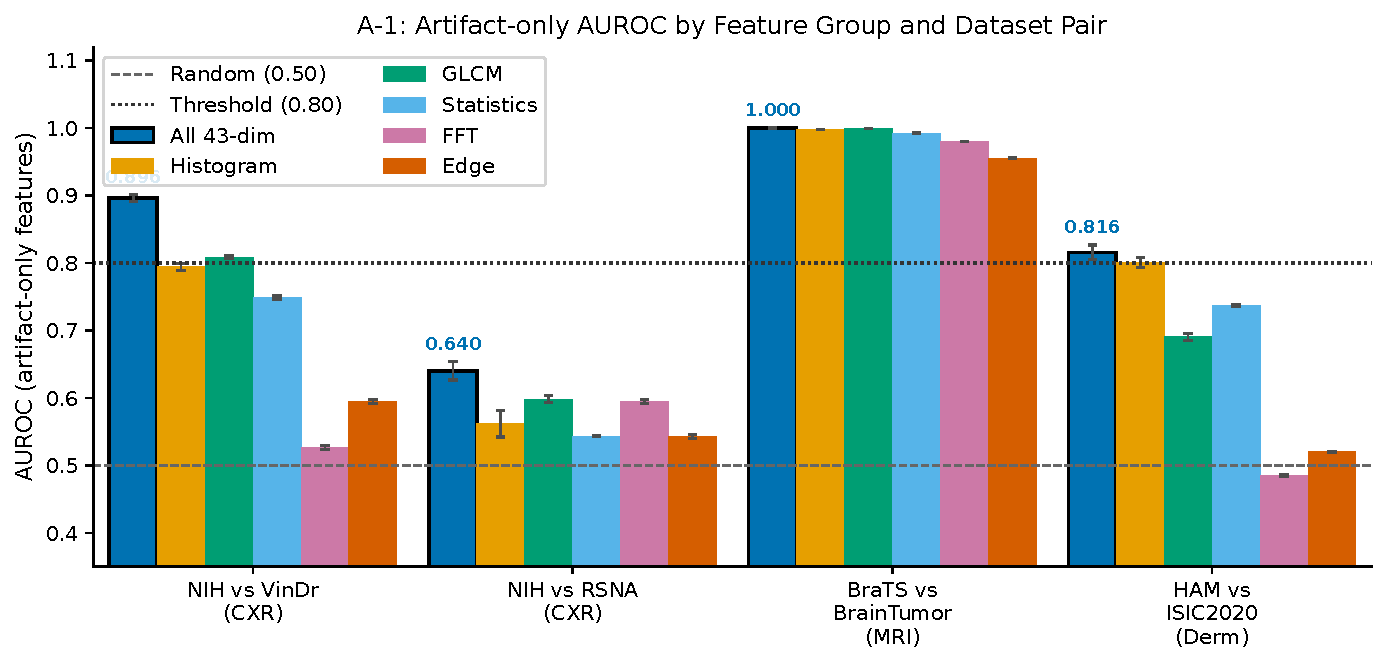
\includegraphics[width=0.78\linewidth]{../figures/fig_a1_artifact_auroc.pdf}
  \caption{Artifact-only white-box localization (A-1/A-2). Content-blind
  43-dimensional features separate source identity at high AUROC across
  cross-institution pairs spanning three modalities, with the per-feature-group
  contributions shown. The signal is localized to concrete physical descriptors
  (histogram, texture, vignetting, spectrum) rather than treated as a black box.}
  \label{fig:a1}
\end{figure}

\subsection{Frozen encoder and OOD detector pool}

For the post-hoc detectors we use a TorchXRayVision DenseNet121-res224 as a
frozen encoder (no fine-tuning, no re-training). From each image we cache (a) the
1024-dimensional penultimate-layer feature and (b) the 18 multi-label disease
logits. All detectors operate on these cached representations except where a live
forward pass is required (noted below).

We evaluate \textbf{13 post-hoc OOD detectors} from OpenOOD, each with its
official hyperparameters. The reused set of seven is: MSP (no parameters); ODIN
($T=1000$, $\epsilon=0.0014$); Energy/EBO ($T=1$); Mahalanobis/MDS (no
parameters); KNN ($K=50$); ViM ($\text{dim}=512$); and GradNorm (no parameters).
For ViM we set $\text{dim}=512$ following the original ViM
paper~\citep{wang2022vim}, whose rule for $N<1500$ penultimate dimensions is
$D \approx N/2$; we annotate this choice explicitly, since OpenOOD provides no
DenseNet121-specific ViM configuration. The extended set of six is: Residual
($\text{dim}=512$, a pure subspace-geometric residual that does not depend on
logits); SHE (inner-product metric); NNGuide ($\alpha=0.01$, $K=100$); fDBD
(\texttt{distance\_as\_normalizer=True}); ASH (percentile $=90$, the only
detector requiring a live forward pass); and DICE ($p=90$).

\paragraph{Detectors we explicitly exclude, and why (not a competitive
selection).} GEN, KLM, Relation, RankFeat, and SCALE are omitted because they
are \emph{architecturally incompatible with this backbone}, not because they
performed worse. They softly depend on a single-label softmax probability
structure, or require intermediate convolutional-layer activations that this
frozen penultimate-plus-classifier setup does not expose. We state this exclusion
criterion before reporting any result, so the pool is not curated post hoc.

\subsection{Multi-label adaptation (frozen, pre-specified)}

The backbone produces 18 multi-label \emph{sigmoid} outputs rather than a
single-label softmax, whereas most OpenOOD post-processors assume single-label
softmax. We therefore pre-specify three adaptations \emph{before running}, and
disclose each as a canonical multi-label generalization together with its
limitation. For SHE, the global pattern is the mean penultimate feature over all
ID images (a single global prototype), scored by inner product; we do not bucket
by pseudo-class, since multi-label data has no single class label and bucketing
would introduce additional degrees of freedom (limitation: this discards
class-conditional structure and measures only global-prototype alignment). For
NNGuide, energy is $\mathrm{logsumexp}$ of the 18 logits, matched to our
Energy/EBO convention; the guide KNN uses $K=100$ cosine similarity (limitation:
under multi-label sigmoid this energy is not a strict free energy and serves only
as a confidence proxy). For DICE / Residual / fDBD, \texttt{get\_fc} reads the
classifier weight $W$ ($18\times1024$) and bias $b$ (18); DICE's mean-activation
sparsification uses ID-train penultimate features at $p=90$ (limitation: the DICE
sparsity mask is defined over the averaged contribution across the 18 sigmoid
heads). Importantly, none of these adapted detectors is allowed to single-handedly
carry our load-bearing source-leakage criterion (see Section~\ref{sec:results});
that criterion is reported for ViM alone, which has no multi-label adaptation
ambiguity (its $\text{dim}=512$ score is a purely geometric residual that does not
depend on a softmax/sigmoid convention).

\subsection{Propensity-matched decontamination}

To remove the part of the ID--OOD gap that hand-crafted artifacts can explain, we
construct an artifact-matched paired subset (the ``cleanC'' subset) and
re-evaluate every detector on it. We match on a 1-dimensional logistic propensity
score with a caliper of $0.2$ standard deviations of the propensity logit,
following the standard meaning of a ``$0.2$~SD caliper'' in the
propensity-score-matching literature~\citep{austin2011caliper,lunt2014caliper}.

We disclose the provenance of this specification openly, because it matters for
reproducibility and for an honest reading of the negative result below. The
matching radius ``$0.2$~SD'' was \emph{pre-registered before any run}. An initial
implementation mistakenly interpreted it as a $0.2\sqrt{43}$ Euclidean ball in
the raw 43-dimensional artifact space; under that curse-of-dimensionality
reading, the most-similar chest-X-ray pair matched only about 6 of 500
candidates, leaving the comparison statistically powerless. We corrected the
implementation to the standard 1-dimensional propensity-logit caliper of
Austin~\citep{austin2011caliper}. This correction \emph{does not bias toward a
positive result}: the pre-correction failure was a no-power failure (bootstrap CI
upper bound $=1.0$), and restoring power could equally have yielded a pass or a
genuine fail.

The seven specifications of the propensity procedure are frozen to prevent
post-hoc degrees of freedom: (1) the propensity model is plain logistic
regression on the same z-scored 43-dimensional artifact features, with no
interaction or polynomial terms; (2) no regularization (or a fixed L2 with the
$\lambda$ stated in text if numerically required; no cross-validated $\lambda$
selection); (3) $k=5$ out-of-fold cross-fitting to prevent self-matching;
(4) caliper $= 0.2 \times \mathrm{SD}(\text{propensity logit})$, pooled;
(5) $1{:}1$ greedy matching without replacement, random order seed $=42$;
(6) a hard floor of $n_\text{matched} \ge 30$ (any pair below this is excluded
from the decontaminated analysis); and (7) mandatory balance diagnostics, with
standardized mean differences (SMD) reported and $|\text{SMD}|<0.1$ the
conventional balance target.

\subsection{Held-out evaluation protocol (the corrected scoring split)}
\label{sec:heldout}

A subtle but consequential point concerns \emph{how} each detector's AUROC is
computed. Several post-hoc detectors---most importantly the \emph{projection-based}
ones (ViM, Residual), and to a lesser degree the distance-based ones (MDS,
KNN)---must first \emph{fit} a representation of the ID class (a principal
subspace, a class mean, a neighbour set) before scoring test points. The standard
protocol for these detectors, as specified in the original ViM
paper~\citep{wang2022vim} (where the principal space $P$ and the parameter
$\alpha$ are determined in advance from the training set) and enforced by
OpenOOD, is to fit on a training set disjoint from the evaluation set. If instead
the same ID samples used to fit that representation also appear as the ID half of
the test set (an \emph{in-sample} evaluation), the fit is evaluated on data it
has already seen, and the resulting AUROC can be inflated in a way that has
nothing to do with the OOD signal under study. This is a known form of
estimation/in-sample leakage; our contribution is not to discover that held-out
fitting is required, but to quantify how severely this known leakage is
\emph{amplified} in the underdetermined regime below.

The risk is acute for projection-based residuals: with only $N_\text{id} \approx
500$ ID samples but a $D = 1024$-dimensional penultimate space, the fitted
principal subspace does not span the ID data, so the in-sample ID residual
collapses to $\approx 0$ while any held-out point has a strictly positive
residual---perfectly separating ``in-sample versus held-out'' rather than
``source A versus source B.'' We note that this $N_\text{id} \approx 500$ is the
size of \emph{our evaluation subset per pair}, not the much larger training set
the ViM paper recommends for fitting the principal space; the $N_\text{id} < D$
condition that triggers this null-space effect is therefore a property of our
per-pair evaluation budget, which we state honestly because it is precisely the
condition under which the amplification arises.

We therefore evaluate every detector under a \textbf{held-out protocol}. The ID
samples of each pair are split (seed $=42$, $0.5$) into a \emph{fit} half and an
\emph{evaluation} half. Each detector is fit \emph{only} on the ID fit half;
AUROC is then computed over $\mathrm{concat}(\text{ID-eval}, \text{OOD})$, so
that no ID sample is ever both fitted and scored. The cleanC (decontaminated)
variant matches within the ID-eval $\times$ OOD subset under the same propensity
caliper. We additionally retain the in-sample path purely as a contrast, because
the \emph{gap between the two protocols is itself a finding} (see
Section~\ref{sec:results}). All load-bearing source-leakage numbers in this paper
are reported under the held-out protocol.

We sanity-check the protocol with a small battery of source-matched negative
controls: (C1) a \emph{same-source} pair (one institution split in half) scored
in-sample, which---if the in-sample artifact is real---should itself spuriously
yield ViM $\approx 1.0$; (C2) the same same-source pair scored held-out, which
should yield AUROC $\approx 0.5$ (no signal, as expected); and (C3) a
\emph{cross-source} pair scored held-out, which isolates the genuine source
signal. The observed pattern (C1 $\approx 1.0$, C2 $\approx 0.5$, C3 well above
$0.5$ but not perfect) confirms that the in-sample $1.0$ originates from the
evaluation asymmetry, not from source covariate, and that a real but moderate
source signal remains under the held-out protocol.

%==============================================================================
\section{Results}
\label{sec:results}
%==============================================================================

\subsection{Artifact-only white-box localization (A-1 / A-2)}

We first establish that the spurious signal can be localized with a content-blind
feature battery (Figure~\ref{fig:a1}). On cross-institution pairs, the
43-dimensional artifact-only features---which never read any pathological
content---separate the two sources at AUROC in the range $0.82$--$0.9997$ on the
load-bearing pairs, spanning all three modalities (chest X-ray, brain MRI,
dermoscopy). The weakest pair, two same-country (US) chest X-ray sources (NIH vs
RSNA), still reaches artifact-only AUROC $=0.64$---lower precisely because the
two sources are physically closer---and we report it openly rather than dropping
it. This satisfies the pre-registered acceptance criteria A-1 ($\ge 2$ of $\ge 3$
pairs at AUROC $\ge 0.80$, with $\ge 1$ pair $>0.90$) and A-2 (each modality has
$\ge 1$ pair at AUROC $>0.75$). In other words, a substantial part of what these
benchmarks present as an ``OOD signal'' is a scanner/institution acquisition
fingerprint that a model never needs to look at the anatomy to read. We do not
claim the signal is \emph{entirely} artifactual; we claim that benchmark
performance is \emph{primarily driven by source separability}, a claim made
precise by the pure-covariate split and the source-distance analysis below.

\subsection{The pure-covariate construction and the in-sample evaluation trap}

Our evidence for source leakage comes from a physically clean construction:
cross-source normal-versus-normal pairs. In each such pair, both sides contain
only normal (non-pathological) images, so there is no semantic (pathology)
difference whatsoever; the \emph{only} systematic difference between the two
sides is the acquisition source. Any detector that separates such a pair is, by
construction, detecting \emph{where the data came from}, not \emph{whether it is
abnormal}.

A pre-registered analysis (criterion A-5) had set out to test whether the
projection-based detector ViM separates these pairs near-perfectly. Under the
common in-sample evaluation, ViM appears to do exactly that---raw AUROC $=1.0$ on
all 7/7 pairs. \textbf{This number, however, is an evaluation artifact, not a
measure of source leakage.} As detailed in Section~\ref{sec:heldout}, the
in-sample protocol lets the ID half of the test set coincide with ViM's fit set;
with $N_\text{id} \approx 500$ ID samples in a $D = 1024$-dimensional space, the
fitted principal subspace does not span the ID data, the in-sample ID residual
collapses to $\approx 0$, and ViM perfectly separates ``in-sample versus
held-out''---\emph{independently of source}. Three negative controls confirm this
directly: a same-source pair (a single institution split in half, with no source
difference at all) scored in-sample \emph{also} yields ViM $=1.0$, while the same
pair scored held-out yields $\approx 0.5$. The $1.0$ is therefore a property of
the evaluation asymmetry, not of the data's source.

\begin{figure}[t]
  \centering
  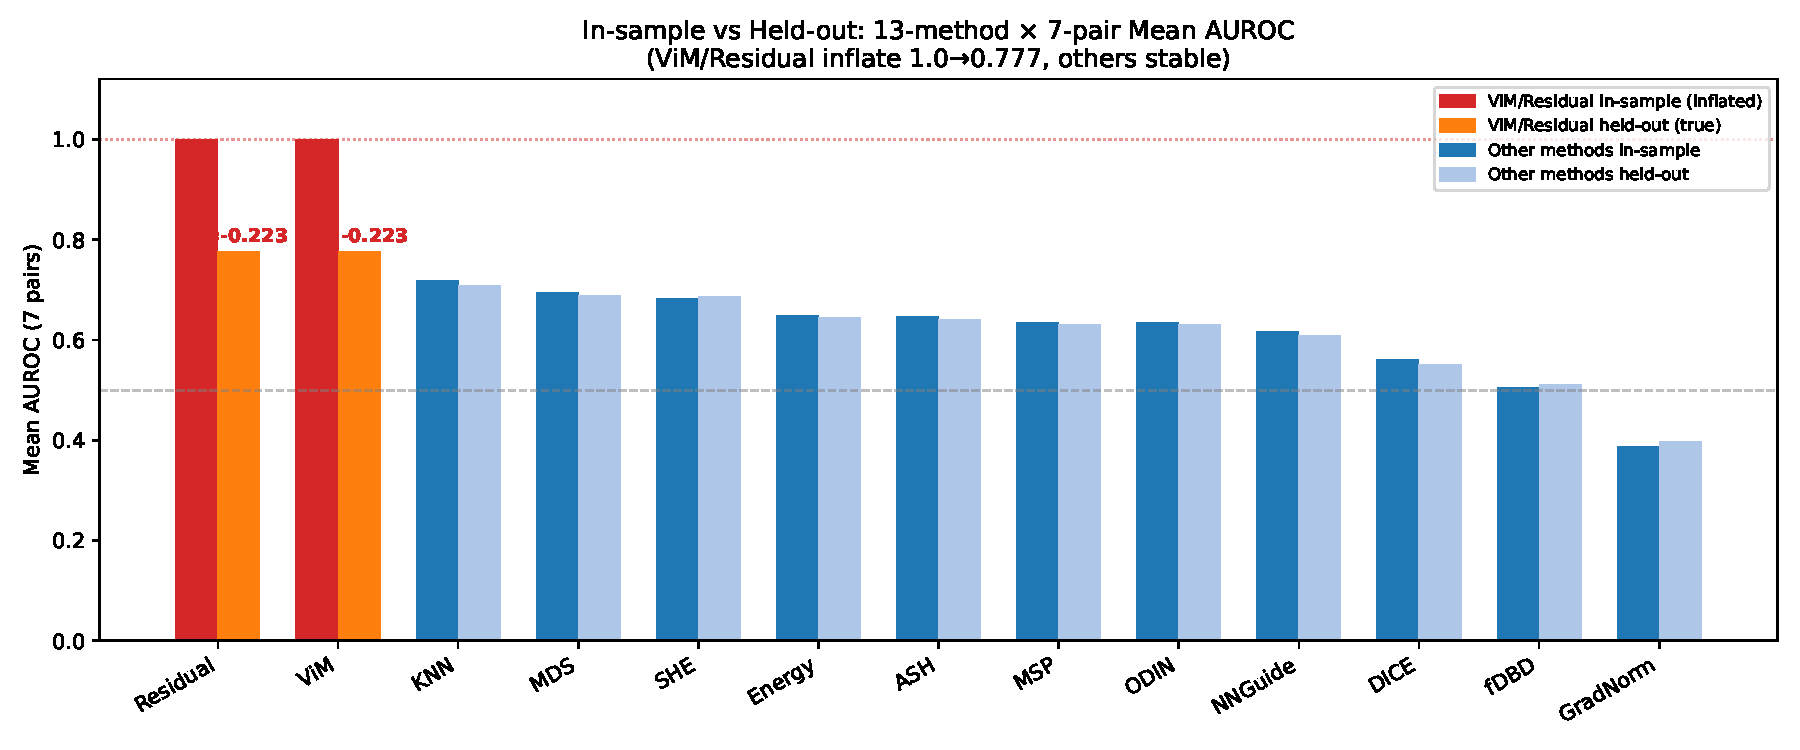
\includegraphics[width=0.72\linewidth]{../figures/fig_heldout_insample_delta.pdf}
  \caption{In-sample evaluation inflation (A-7). The gap
  $\Delta = (\text{in-sample} - \text{held-out})$ AUROC is sharply localized to
  the projection-based detectors (ViM and Residual, $+0.223$ each, falling from
  $1.00$ to $0.777$); for all eleven other detectors $|\Delta| < 0.012$. The same
  \emph{known} estimation leakage inflates AUROC by less than $0.005$ in the
  conventional $N \gg D$ regime; in the $N_\text{id} < D$ underdetermined
  subspace it is amplified to a deterministic perfect separation that masquerades
  as a flawless source-leakage result.}
  \label{fig:delta}
\end{figure}

\paragraph{In-sample evaluation inflation (A-7, a methodological finding).} We
are precise about what is and is not new here. Held-out fitting is \emph{not} our
discovery: it is the standard protocol of ViM~\citep{wang2022vim} and
OpenOOD~\citep{yang2022openood}, and an in-sample fit is a known form of
estimation leakage. What we contribute is a quantification of how severely this
known leakage is amplified in a specific, common-in-practice regime---an
underdetermined projection subspace ($N_\text{id} < D$) on cross-source medical
benchmarks---and of how precisely it can masquerade as a credible benchmark
conclusion. The size of the inflation is sharply localized to the
projection-based detectors, which makes the mechanism clean
(Figure~\ref{fig:delta}). The gap $\Delta = (\text{in-sample} - \text{held-out})$
AUROC is $+0.223$ for ViM and $+0.223$ for Residual (each falling from $1.00$ to
$0.777$), but $|\Delta| < 0.012$ for all eleven other detectors, which do not fit
a low-rank ID subspace. For calibration, the general
leakage taxonomy~\citep{roth2026leakage} documents that in-sample estimation
leakage typically inflates AUROC by less than $0.005$ in the conventional
$N \gg D$, low-dimensional regime; here, in the $N_\text{id} < D$ underdetermined
subspace, the \emph{same} leakage is amplified by an order of magnitude
($+0.223$) and---decisively---it does not merely add noise but produces a
\emph{deterministic} perfect separation (AUROC $=1.0$) that mimics a flawless
source-leakage result, convincing enough to pass a pre-submission self-review.
This packaged ``$N_\text{id} < D$ amplification $+$ masquerade as a credible
source-leakage benchmark-critique'' is, to our knowledge, not isolated in the
prior literature, and it is the central cautionary methodological contribution of
this paper. We present it as a finding and a cautionary tale, not as an
implementation bug, and we do \emph{not} claim to have discovered that
projection-based detectors require held-out evaluation.

\subsection{Source leakage under the corrected held-out protocol}

Re-scored under the held-out protocol, the genuine source signal is \emph{real
but moderate, and it is driven by how far apart the two sources are}. ViM's
held-out AUROC across the seven pairs is reported in Table~\ref{tab:heldout}.

\begin{table}[t]
  \centering
  \caption{ViM AUROC under the corrected held-out protocol, the (artifactual)
  in-sample value, and the artifact-only separability, for the seven cross-source
  normal-versus-normal pairs. Mean held-out ViM AUROC $=0.777$. NIH vs RSNA is a
  deliberately reported honest negative case (held-out ViM $\approx$ chance).}
  \label{tab:heldout}
  \begin{tabular}{lccc}
    \toprule
    Pair & Held-out ViM & In-sample (artifact) & Artifact-only \\
    \midrule
    BraTS vs BrainTumor (MRI)        & 0.997 & 1.0 & 0.9997 \\
    HAM vs fitzpatrick17k (derm)     & 0.938 & 1.0 & 0.991  \\
    NIH vs VinDr (CXR)               & 0.841 & 1.0 & 0.896  \\
    ISIC2020 vs PAD-UFES (derm)      & 0.798 & 1.0 & 0.805  \\
    VinDr vs RSNA (CXR)              & 0.772 & 1.0 & 0.907  \\
    HAM vs ISIC2020 (derm)           & 0.689 & 1.0 & 0.816  \\
    \textbf{NIH vs RSNA (honest negative)} & \textbf{0.406} & 1.0 & 0.640 \\
    \bottomrule
  \end{tabular}
\end{table}

The mean held-out ViM AUROC is $0.777$. Every value sits above the same-source
held-out chance level of $\approx 0.5$ except the deliberately reported negative
case, so a real source signal does exist; but it is \emph{far from the perfect
separation the in-sample number suggested}, and it clears the pre-registered
strict A-5 bar (ViM $>0.95$ on $\ge 6/7$ pairs) on only $2/7$ pairs (BraTS and
HAM-vs-fitzpatrick17k). We therefore record A-5 as a \emph{pre-registered FAIL}
under the corrected protocol and, following the pre-specified fallback, move the
load-bearing weight to A-1/A-2 (phenomenon), A-7 (mechanism), and A-6
(prescription).

\paragraph{Source distance is a major driver of the spread.} With the
artifact-only reference completed for all seven pairs ($n=7$), the held-out ViM
AUROC tracks artifact-only separability strongly: Spearman $\rho = 0.821$ and
Pearson $r = 0.955$ (Figure~\ref{fig:vim-vs-artifact}). The more physically
distinct the two sources, the more the detector can read; the more similar they
are, the less. We characterize source distance as \emph{a major driver} rather
than the sole factor: a perfectly monotone rank correspondence on only four
reference pairs has a non-negligible chance probability ($\approx 8.3\%$), so we
deliberately completed all seven references and report the resulting
$\rho = 0.821$ honestly, rather than the artificially tidy $\rho = 1.0$ that the
four-point subset alone would have suggested. The relationship also yields an
\emph{honest negative example within the same modality}: NIH vs RSNA, two US
chest-X-ray sources, has the lowest artifact-only separability ($0.64$) and a
held-out ViM of $0.406$, indistinguishable from chance. This single point is
decisive evidence \emph{against} over-claiming: source leakage is not a universal
property of the modality or the detector---it scales with source distance, and it
can vanish entirely when the two institutions are acquisition-similar.

\begin{figure}[t]
  \centering
  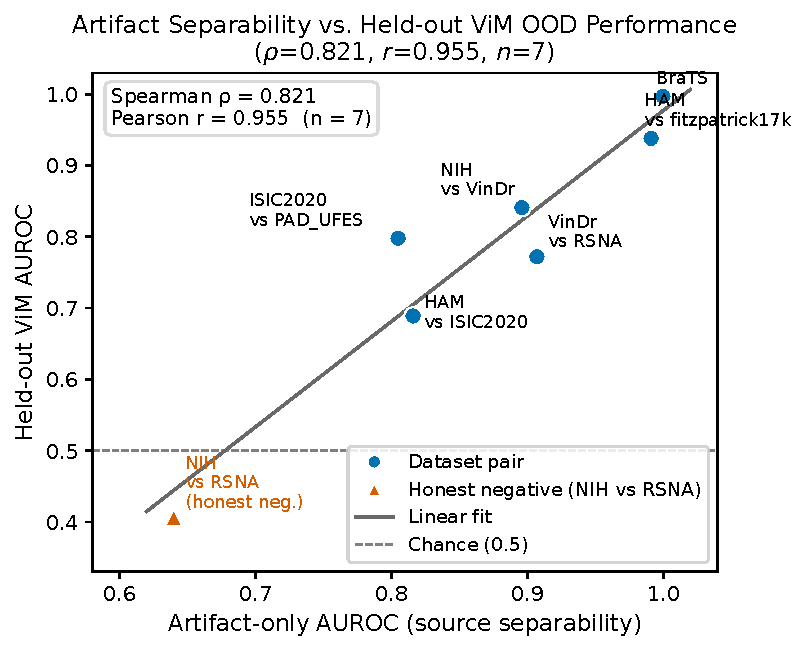
\includegraphics[width=0.62\linewidth]{../figures/fig_heldout_vim_vs_artifact.pdf}
  \caption{Held-out ViM AUROC versus artifact-only separability across the seven
  cross-source pairs ($n=7$). The two track strongly (Spearman $\rho = 0.821$,
  Pearson $r = 0.955$): source distance is a major driver of the spread. The
  honest negative case (NIH vs RSNA: artifact $0.64$, held-out ViM $0.406 \approx$
  chance) anchors the lower-left.}
  \label{fig:vim-vs-artifact}
\end{figure}

\subsection{The 13-detector held-out spectrum: heterogeneity reported as-is}

Under the held-out protocol, mean AUROC across the 13 detectors is heterogeneous
and, again, modest (Figure~\ref{fig:heatmap}): ViM and Residual (the
projection-based pair) at mean $0.777$; a middle band of KNN ($0.709$), MDS
($0.688$), and SHE ($0.686$); a logit-based band at roughly $0.61$--$0.64$; and a
weak tail of DICE ($0.551$), fDBD ($0.510$), down to GradNorm at $0.397$, the
lowest of all 13 and the only gradient-dependent detector---under a frozen
encoder it cannot capture the source covariate. The leakage is likewise not
uniform across pairs: on the well-separated BraTS pair, 8 of 13 detectors exceed
$0.75$, whereas on the acquisition-similar NIH-vs-RSNA pair, 8 of 13 fall below
$0.55$.

We report this spectrum \emph{descriptively only}, and we deliberately do
\emph{not} attach any group-level claim (such as ``feature-based detectors
systematically beat logit-based detectors''): a leave-ViM-out check showed that
such a group-level effect reverses sign on chest X-ray once ViM is removed, i.e.\
the apparent regularity was essentially carried by ViM alone. We present the
heterogeneity itself, and the breadth of the detector pool, as
artifact-completeness evidence, without over-claiming a structure that does not
survive its own robustness check.

\begin{figure}[t]
  \centering
  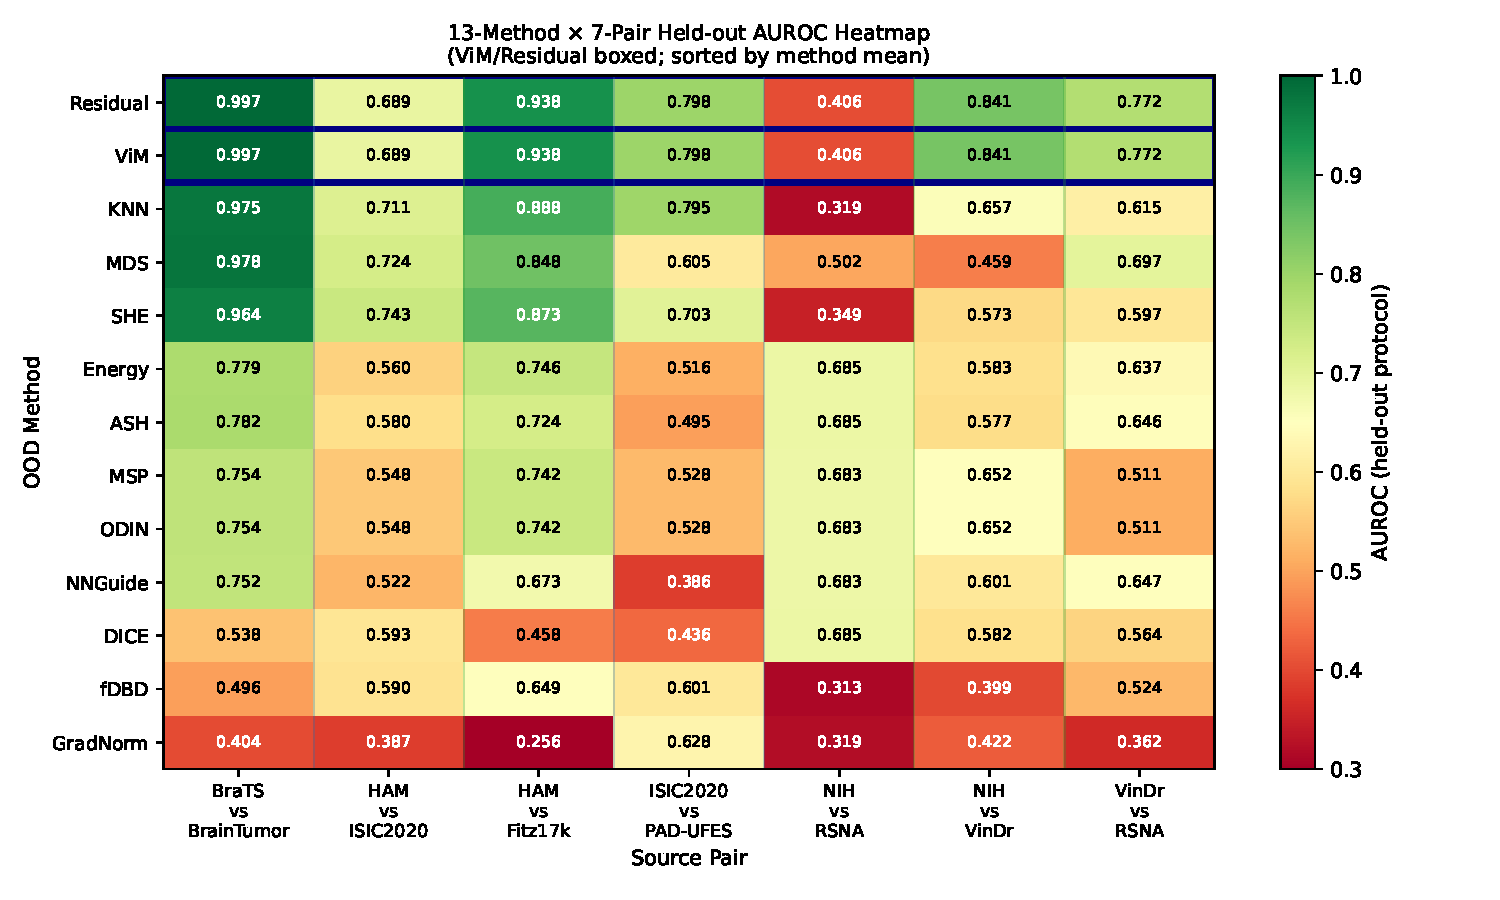
\includegraphics[width=0.86\linewidth]{../figures/fig_heldout_heatmap_13x7.pdf}
  \caption{Held-out AUROC for all 13 detectors $\times$ 7 cross-source pairs. The
  leakage is heterogeneous across both detectors and pairs and, overall, modest;
  it is strongest on the well-separated BraTS pair and weakest on the
  acquisition-similar NIH-vs-RSNA pair. We report the full spectrum descriptively
  and attach no group-level claim.}
  \label{fig:heatmap}
\end{figure}

\subsection{The pre-registered ranking-flip criterion (A-4): an honest negative
result}

We had pre-registered a \emph{different} criterion as the original single
load-bearing test: whether decontamination changes the ranking of OOD detectors.
The pass condition was specified in advance as a conjunction (an AND gate): the
bootstrap CI upper bound of the Spearman correlation between the original and
decontaminated rankings must fall below $0.7$ \emph{or} the top-1 detector must
drop out of the top-3, \emph{and} the observed re-ranking must be mechanistically
consistent with the pre-registered detector-sensitivity ordering
($\text{MDS} > \text{KNN/ViM} > \text{MSP}$). Under the corrected held-out
protocol, of the seven cross-source pairs, \emph{five are evaluable} (the BraTS
pair and the HAM-vs-fitzpatrick17k pair are INSUFFICIENT, with
$n_\text{matched} = 8$ and $26$ respectively, both below the $n \ge 30$ floor).
Of the five evaluable pairs, \emph{four FAIL and one genuinely PASS}.

The four failing pairs are NIH-vs-VinDr (Spearman point estimate $0.9725$, CI
upper bound $1.0$), NIH-vs-RSNA ($0.967$, CI upper bound $1.0$), VinDr-vs-RSNA
($0.9396$, CI upper bound $1.0$), and ISIC2020-vs-PAD-UFES ($0.6374$, CI upper
bound $0.9145$---the smallest upper bound among all evaluable pairs). In none of
these does the ranking flip survive its bootstrap CI.

The single passing pair is \textbf{HAM-vs-ISIC2020 (dermoscopy)}. Here the
pre-registered pass condition is genuinely met: the top-1 detector, SHE, drops
from rank 1 to rank 6 after decontamination---i.e.\ out of the top-3---while the
second mechanistic caliper is also satisfied (the re-ranking under the second
readout has Spearman $1.0$, matching the pre-registered sensitivity-ordering
hypothesis $\text{MDS} > \text{KNN/ViM} > \text{MSP}$). The point estimate of the
AND gate's first caliper for this pair is Spearman $0.3736$ with a CI upper bound
of $0.9446$. We report this PASS honestly: under the held-out protocol, one of
five evaluable pairs \emph{does} trigger the pre-registered ranking flip.

We are equally careful not to over-read this single PASS. The bootstrap CI on the
ranking-flip statistic is extremely wide for this pair (for example, the
HAM-vs-ISIC2020 Spearman CI spans $[-0.24, 0.94]$), which is the signature of a
\emph{structurally low-power} test: with only a handful of rank points the
bootstrap Spearman CI is intrinsically near-saturated on $[-1, 1]$, so an upper
bound below $0.7$ is nearly unreachable and the criterion can FAIL---or,
occasionally, PASS through the top-1-drop disjunct---essentially independently of
the underlying truth. Expanding the detector pool from 7 to 13 did not rescue the
test's power, consistent with this analysis. A single 1-of-5 PASS under such low
power is therefore far too thin to support a general, actionable ``decontamination
flips the ranking'' claim. We keep both the four FAILs and the one PASS on the
record---neither deleting the negative result nor inflating the lone
positive---and treat the criterion's structural low power itself as a finding
useful to the community. (An earlier in-sample reading of this same matrix
reported a uniform failure; the held-out re-analysis above supersedes it, and the
single held-out PASS is reported in place of that earlier all-FAIL summary.)

%==============================================================================
\section{Discussion and Limitations}
%==============================================================================

\subsection{How this artifact survived two independent audits (a credibility
argument)}

Before recounting the development history, we make one structural point that
frames everything below. The phenomenon-level results (A-1/A-2, the artifact-only
white-box localization) are \emph{fully independent of the projection-based
geometric scoring chain that the history below overturns}. Artifact-only AUROC is
computed from a 43-dimensional hand-crafted feature battery with a simple
held-out classifier; it never fits a ViM principal subspace, never touches the
penultimate-space null-space residual, and is therefore structurally immune to
the in-sample inflation that contaminated the ViM numbers. The reader should not
transfer any doubt about the corrected ViM chain onto A-1/A-2: the two evidence
streams do not share the failure mode. With that established, we recount the
history not as a confession of mistakes, but as evidence that \emph{this
benchmark instrument can falsify its own headline number under two independent
audits---a positive signal for its trustworthiness}, since a critique tool that
cannot detect its own contamination is of little use as a critique tool.

We are explicit about the order in which this work developed, so that the reader
can verify we are not retrofitting a hypothesis to the data. \emph{First}, a
single criterion was pre-registered before any run: A-4, the ranking-flip test,
was frozen as the sole load-bearing criterion, with its pass condition fixed in
advance. \emph{Second}, A-4 was run and, under the corrected held-out protocol,
did not support an actionable ranking-flip claim: of five evaluable pairs, four
FAIL and only one (HAM-vs-ISIC2020, dermoscopy) triggers the pre-registered
flip---and that lone PASS sits under a structurally low-power test whose bootstrap
CI is too wide (e.g.\ $[-0.24, 0.94]$ for that pair) to carry a general claim. We
kept both the four failing pairs and the single passing pair on the record,
declined to elevate a 1-of-5 result into a headline, downgraded the criterion to
a negative-leaning result, and elevated the structural-low-power analysis itself
into a contribution. (Under the alternative in-sample protocol the same criterion
failed uniformly; neither protocol yields a general ranking-flip claim.)
\emph{Third}, we reframed the headline onto a source-leakage criterion (A-5) and,
on the in-sample protocol, observed ViM AUROC $=1.0$ on all 7/7 pure-covariate
pairs.

That number was then caught by two independent audits, and we report both in
full. The first audit was pre-registered self-scrutiny: an adversarial review of
our own draft flagged that ViM $=1.0$ could be a trivial evaluation artifact
rather than a genuine source covariate. The second was an in-sample falsification
by negative control: we wrote source-matched negative controls and confirmed
exactly that---a same-source pair (a single institution split in half, with no
source difference at all) scored in-sample \emph{also} yields $1.0$, so the
perfect separation came from the in-sample fit/evaluation overlap, not from
source. Having been falsified twice, the number was corrected: we re-ran the
entire matrix under the standard held-out protocol; the true ViM values are
$0.406$--$0.997$ (mean $0.777$, $>0.95$ on only $2/7$ pairs), so the strict A-5
bar fails, and we say so. Following the pre-specified fallback, we moved the
load-bearing weight to the three results that \emph{do} hold honestly:
artifact-only localization (A-1/A-2, phenomenon, independent of the overturned
chain as noted above), the in-sample-inflation quantification (A-7, mechanism),
and the evaluation prescription (A-6). We state plainly that the headline was
reframed and that the original ``ViM $=1.0$ perfect source leakage'' claim was a
self-corrected in-sample artifact; we do not pretend this was always the claim.
Crucially, the held-out protocol we corrected \emph{to} is the standard protocol
of ViM and OpenOOD, not a protocol we invented---so the contribution of A-7 is
not ``we discovered held-out evaluation,'' but the quantification of how a
\emph{known} leakage is amplified to a deterministic perfect separation under
$N_\text{id} < D$ and masquerades as a credible benchmark conclusion. The
in-sample inflation is reported as a finding and a cautionary methodological
contribution---a pitfall any practitioner can fall into, and one our own
instrument detected---rather than as a defect we apologize for.

\subsection{Deep source leakage outruns hand-crafted matching (a double-edged
disclosure)}

Our most consequential limitation is also a finding, and we disclose it rather
than letting a reviewer discover it. The propensity-matched decontamination
removes the covariate component that the 43 hand-crafted artifact features can
explain (artifact-only AUROC drops below $0.65$ on the matched subset). Yet under
the held-out protocol ViM still attains AUROC $=0.628$ on the decontaminated
(cleanC) subset, down only modestly from its held-out raw value of $0.777$
($\Delta = -0.149$) and still above the $\approx 0.5$ chance level. The
implication cuts both ways. As a \emph{finding}, it qualifies the source-leakage
account honestly: ViM's virtual-logit residual captures a backbone-internal
source representation that is partly beyond the reach of hand-crafted
matching---propensity matching on 43 hand-crafted features removes only a fraction
of it. As a \emph{limitation}, it bounds our decontamination protocol: deep
source leakage is not fully removable by 43-dimensional hand-crafted matching, so
our protocol cannot claim to eliminate it. We report both faces. (We note that an
earlier draft reported cleanC ViM $=1.0$; that figure was the same in-sample
artifact corrected above, and the honest held-out value is $0.628$.)

\subsection{Matching balance, disclosed in full}

The held-out source-leakage AUROCs are measured on the held-out \emph{raw}
ID/OOD split and are structurally independent of the quality of any matched
subset; only the \emph{decontaminated} (cleanC) and ranking-flip (A-4) readings
depend on matching. This matters for the pairs with imperfect balance. We report
SMDs in full: across the matched pairs $\text{SMD}_\text{max}$ exceeds the
conventional $0.1$ target even where $\text{SMD}_\text{mean}$ stays below $0.1$,
and one dermoscopy pair (HAM vs fitzpatrick17k, $n=39$) has
$\text{SMD}_\text{max} = 0.675$, a genuinely poor balance. We disclose this
openly. It constrains the cleanC and A-4 readings for that pair, but it does
\emph{not} touch the held-out raw source-leakage values, which never use that
pair's matched subset.

\subsection{A prescription for evaluation (A-6)}

The actionable consequence of this work is a small, concrete evaluation
prescription that does not rely on the low-power ranking-flip test.

\begin{enumerate}
  \item \textbf{Use a cross-source normal-versus-normal pair as a sanity
  baseline.} If a detector scores a high AUROC on such a pair---where there is no
  pathology difference to detect---then the benchmark is contaminated by source
  separability, and its OOD results on that pair should be read as, at least in
  part, source detection rather than abnormality detection.
  \item \textbf{Report the artifact-only AUROC as a contamination upper bound}
  for any benchmark pair, quantifying how source-separable that pair is before
  any detector is even applied.
  \item \textbf{For projection-based / subspace-residual detectors (e.g.\ ViM,
  Residual), explicitly state the fit/evaluation split in any reported AUROC.}
  Held-out fitting is already the standard protocol for these detectors (ViM,
  OpenOOD), so we do not present ``use held-out'' as a discovery; the actionable
  warning is sharper. When the ID fit set overlaps the ID evaluation set (an
  in-sample misuse), and the ID sample count is below the feature dimension
  ($N_\text{id} < D$, as in per-pair medical evaluation budgets), the inflation
  is not a mild, noisy bias but a \emph{deterministic perfect separation} (here, a
  $+0.223$ AUROC inflation localized to ViM/Residual, driving them to AUROC
  $=1.0$) that closely mimics a genuine source-leakage result and can pass a
  casual self-review. Reviewers and practitioners should therefore treat a
  near-perfect AUROC from such a detector as a red flag prompting an explicit
  check of the fit/evaluation split, rather than as a strong result.
\end{enumerate}

Together these turn the present diagnosis into a reusable evaluation protocol: a
benchmark that fails the sanity baseline is announcing that, for
cross-institution pairs, ``a stronger OOD detector'' may simply be ``a detector
that reads source fingerprints better''---or, worse, one that reads an in-sample
geometric artifact.

\subsection{Scope and what we do not claim}

We do not claim that \emph{all} OOD benchmarks are invalid, nor that source
leakage is perfect or universal. We claim that \emph{when ID and OOD are drawn
from different institutions---as in most medical OOD benchmarks---method
performance is confounded by source separability, in proportion to how far apart
the two sources are}, and that this confound should be checked with a cross-source
normal-versus-normal sanity baseline (evaluated held-out) and bounded with an
artifact-only contamination upper bound. The held-out source signal is real but
moderate (mean ViM AUROC $0.777$) and can vanish entirely between
acquisition-similar sources (NIH vs RSNA, $0.406 \approx$ chance). We also do not
claim to have discovered that projection-based detectors require held-out
fitting---that is their standard protocol; our A-7 contribution is the
quantification of how a known in-sample estimation leakage is amplified to a
deterministic perfect separation under $N_\text{id} < D$ and masquerades as a
credible source-leakage result. The in-sample-inflation quantification, the
ranking-flip negative result (four FAILs and a single low-power PASS), the
partial removability of deep leakage, and the matching-imbalance disclosures
above are all part of an honest accounting of where this protocol is strong and
where it is bounded.

%==============================================================================
\section{Conclusion}
%==============================================================================

We audited what existing OOD detectors actually measure on cross-institution
medical-imaging benchmarks. A content-blind artifact-only feature battery
localizes the spurious signal to concrete acquisition descriptors and separates
source identity at high AUROC across three modalities; the genuine source signal,
measured under the correct held-out protocol, is real but moderate (mean ViM
AUROC $0.777$) and scales with source distance, vanishing entirely between
acquisition-similar institutions. Along the way we quantified how a known
in-sample estimation leakage is amplified, in the underdetermined
$N_\text{id} < D$ projection subspace, into a deterministic perfect separation
that masquerades as a flawless source-leakage result---and we report the
self-correction of our own headline as evidence that the instrument can falsify
itself. From this diagnosis we distill a portable evaluation prescription: a
cross-source normal-versus-normal sanity baseline, an artifact-only contamination
upper bound, and explicit fit/evaluation split reporting for projection-based
detectors. We hope these turn a cautionary tale into a reusable safeguard for the
community.

%==============================================================================
\bibliographystyle{plainnat}
\bibliography{refs}
%==============================================================================

\end{document}
